%!TEX root = Problems1_main.tex

% Remove the author and date fields and the space associated with them
% from the definition of maketitle!
\makeatletter
\renewcommand{\@maketitle}{
\newpage
 \null
 \vskip 2em%
 \begin{center}%
  {\Large \@title \par}%
 \end{center}%
 \par} \makeatother

\begin{center}
\Huge University Physcis Problems 1\\[1em]
\large 23rd January 2013
\end{center}

\section{Rolling}
Two balls of identical mass and shape with coefficient of friction $\mu=0$, are set rolling at the same initial velocity from point A. Ignoring air resistance, which reaches the end of the track, point B, first and why?
\begin{figure}[ht]
  \centering
  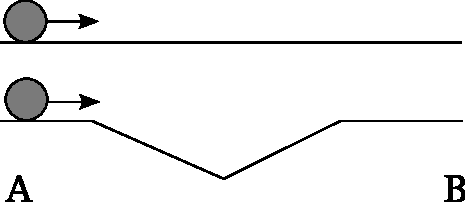
\includegraphics[width=0.4\textwidth]{rolling_balls.pdf}
\end{figure}

\section{Running}
Runners race from point A to point B. The first section is smooth tarmac where there is good grip, the second is soft sand. Which of the five possible paths, a to e, is the fastest and why? Explain your answer.
\begin{figure}[ht]
  \centering
  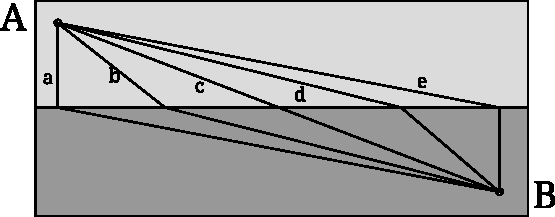
\includegraphics[width=0.6\textwidth]{runners.pdf}
\end{figure}

Which area of physics is the applicable to? How would you solve this numerically?

\section{Dropping}
A slinky is suspended at the top and hangs under its own weight. The top is released. Does the bottom initially:
\begin{enumerate}[label=\alph*)]
	\item move up,
	\item move down,
	\item stay still?
\end{enumerate}

\section{Counting}
Calculate the number of molecules in each of your breaths that was inhaled by Julius Ceasar in his final breath. What assumptions have you made? Use the radius of the earth to be roughly 6\,300\,km.

\section{Floating}
Four vessels each contain a block of floating ice in water. In the first vessel, the ice is solid; in the second, the ice has a large air buble trapped inside; the third has a region of water trapped and the fourth contains a large iron nail.

What happens to the level of the water in each vessel when all the water has melted?
\begin{enumerate}[label=\alph*)]
	\item move up,
	\item move down,
	\item no change?
\end{enumerate}
\begin{figure}[ht]
  \centering
  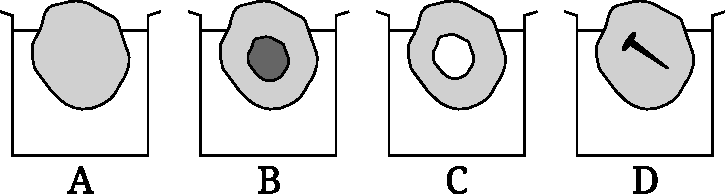
\includegraphics[width=0.8\textwidth]{vessels.pdf}
\end{figure}

\section{Observing}
If you observe an object in a mirror, there is one object and one image. How many images will you observe if two mirrors are placed 
\begin{enumerate}[label=\alph*)]
	\item at 90 degrees to each other,
	\item less than 90 degrees,
	\item greater than 90 degrees?
\end{enumerate}
